% Options for packages loaded elsewhere
% Options for packages loaded elsewhere
\PassOptionsToPackage{unicode}{hyperref}
\PassOptionsToPackage{hyphens}{url}
%
\documentclass[
  14pt,
  ignorenonframetext,
  aspectratio=169,
]{beamer}
\newif\ifbibliography
\usepackage{pgfpages}
\setbeamertemplate{caption}[numbered]
\setbeamertemplate{caption label separator}{: }
\setbeamercolor{caption name}{fg=normal text.fg}
\beamertemplatenavigationsymbolsempty
% remove section numbering
\setbeamertemplate{part page}{
  \centering
  \begin{beamercolorbox}[sep=16pt,center]{part title}
    \usebeamerfont{part title}\insertpart\par
  \end{beamercolorbox}
}
\setbeamertemplate{section page}{
  \centering
  \begin{beamercolorbox}[sep=12pt,center]{section title}
    \usebeamerfont{section title}\insertsection\par
  \end{beamercolorbox}
}
\setbeamertemplate{subsection page}{
  \centering
  \begin{beamercolorbox}[sep=8pt,center]{subsection title}
    \usebeamerfont{subsection title}\insertsubsection\par
  \end{beamercolorbox}
}
% Prevent slide breaks in the middle of a paragraph
\widowpenalties 1 10000
\raggedbottom
\usepackage{iftex}
\ifPDFTeX
  \usepackage[T1]{fontenc}
  \usepackage[utf8]{inputenc}
  \usepackage{textcomp} % provide euro and other symbols
\else % if luatex or xetex
  \usepackage{unicode-math} % this also loads fontspec
  \defaultfontfeatures{Scale=MatchLowercase}
  \defaultfontfeatures[\rmfamily]{Ligatures=TeX,Scale=1}
\fi
\usepackage{lmodern}

\usetheme[]{monash}
\ifPDFTeX\else
  % xetex/luatex font selection
\fi
% Use upquote if available, for straight quotes in verbatim environments
\IfFileExists{upquote.sty}{\usepackage{upquote}}{}
\IfFileExists{microtype.sty}{% use microtype if available
  \usepackage[]{microtype}
  \UseMicrotypeSet[protrusion]{basicmath} % disable protrusion for tt fonts
}{}
\makeatletter
\@ifundefined{KOMAClassName}{% if non-KOMA class
  \IfFileExists{parskip.sty}{%
    \usepackage{parskip}
  }{% else
    \setlength{\parindent}{0pt}
    \setlength{\parskip}{6pt plus 2pt minus 1pt}}
}{% if KOMA class
  \KOMAoptions{parskip=half}}
\makeatother

\usepackage{color}
\usepackage{fancyvrb}
\newcommand{\VerbBar}{|}
\newcommand{\VERB}{\Verb[commandchars=\\\{\}]}
\DefineVerbatimEnvironment{Highlighting}{Verbatim}{commandchars=\\\{\}}
% Add ',fontsize=\small' for more characters per line
\usepackage{framed}
\definecolor{shadecolor}{RGB}{248,248,248}
\newenvironment{Shaded}{\begin{snugshade}}{\end{snugshade}}
\newcommand{\AlertTok}[1]{\textcolor[rgb]{0.94,0.16,0.16}{#1}}
\newcommand{\AnnotationTok}[1]{\textcolor[rgb]{0.56,0.35,0.01}{\textbf{\textit{#1}}}}
\newcommand{\AttributeTok}[1]{\textcolor[rgb]{0.13,0.29,0.53}{#1}}
\newcommand{\BaseNTok}[1]{\textcolor[rgb]{0.00,0.00,0.81}{#1}}
\newcommand{\BuiltInTok}[1]{#1}
\newcommand{\CharTok}[1]{\textcolor[rgb]{0.31,0.60,0.02}{#1}}
\newcommand{\CommentTok}[1]{\textcolor[rgb]{0.56,0.35,0.01}{\textit{#1}}}
\newcommand{\CommentVarTok}[1]{\textcolor[rgb]{0.56,0.35,0.01}{\textbf{\textit{#1}}}}
\newcommand{\ConstantTok}[1]{\textcolor[rgb]{0.56,0.35,0.01}{#1}}
\newcommand{\ControlFlowTok}[1]{\textcolor[rgb]{0.13,0.29,0.53}{\textbf{#1}}}
\newcommand{\DataTypeTok}[1]{\textcolor[rgb]{0.13,0.29,0.53}{#1}}
\newcommand{\DecValTok}[1]{\textcolor[rgb]{0.00,0.00,0.81}{#1}}
\newcommand{\DocumentationTok}[1]{\textcolor[rgb]{0.56,0.35,0.01}{\textbf{\textit{#1}}}}
\newcommand{\ErrorTok}[1]{\textcolor[rgb]{0.64,0.00,0.00}{\textbf{#1}}}
\newcommand{\ExtensionTok}[1]{#1}
\newcommand{\FloatTok}[1]{\textcolor[rgb]{0.00,0.00,0.81}{#1}}
\newcommand{\FunctionTok}[1]{\textcolor[rgb]{0.13,0.29,0.53}{\textbf{#1}}}
\newcommand{\ImportTok}[1]{#1}
\newcommand{\InformationTok}[1]{\textcolor[rgb]{0.56,0.35,0.01}{\textbf{\textit{#1}}}}
\newcommand{\KeywordTok}[1]{\textcolor[rgb]{0.13,0.29,0.53}{\textbf{#1}}}
\newcommand{\NormalTok}[1]{#1}
\newcommand{\OperatorTok}[1]{\textcolor[rgb]{0.81,0.36,0.00}{\textbf{#1}}}
\newcommand{\OtherTok}[1]{\textcolor[rgb]{0.56,0.35,0.01}{#1}}
\newcommand{\PreprocessorTok}[1]{\textcolor[rgb]{0.56,0.35,0.01}{\textit{#1}}}
\newcommand{\RegionMarkerTok}[1]{#1}
\newcommand{\SpecialCharTok}[1]{\textcolor[rgb]{0.81,0.36,0.00}{\textbf{#1}}}
\newcommand{\SpecialStringTok}[1]{\textcolor[rgb]{0.31,0.60,0.02}{#1}}
\newcommand{\StringTok}[1]{\textcolor[rgb]{0.31,0.60,0.02}{#1}}
\newcommand{\VariableTok}[1]{\textcolor[rgb]{0.00,0.00,0.00}{#1}}
\newcommand{\VerbatimStringTok}[1]{\textcolor[rgb]{0.31,0.60,0.02}{#1}}
\newcommand{\WarningTok}[1]{\textcolor[rgb]{0.56,0.35,0.01}{\textbf{\textit{#1}}}}

\usepackage{longtable,booktabs,array}
\newcounter{none} % for unnumbered tables
\usepackage{calc} % for calculating minipage widths
\usepackage{caption}
% Make caption package work with longtable
\makeatletter
\def\fnum@table{\tablename~\thetable}
\makeatother
\usepackage{graphicx}
\makeatletter
\newsavebox\pandoc@box
\newcommand*\pandocbounded[1]{% scales image to fit in text height/width
  \sbox\pandoc@box{#1}%
  \Gscale@div\@tempa{\textheight}{\dimexpr\ht\pandoc@box+\dp\pandoc@box\relax}%
  \Gscale@div\@tempb{\linewidth}{\wd\pandoc@box}%
  \ifdim\@tempb\p@<\@tempa\p@\let\@tempa\@tempb\fi% select the smaller of both
  \ifdim\@tempa\p@<\p@\scalebox{\@tempa}{\usebox\pandoc@box}%
  \else\usebox{\pandoc@box}%
  \fi%
}
% Set default figure placement to htbp
\def\fps@figure{htbp}
\makeatother





\setlength{\emergencystretch}{3em} % prevent overfull lines

\providecommand{\tightlist}{%
  \setlength{\itemsep}{0pt}\setlength{\parskip}{0pt}}



 


% Colors
\definecolor{shadecolor}{RGB}{225,225,225}
\setbeamercolor{description item}{fg=Orange}
\definecolor{MonashBlue}{RGB}{66,109,152}
\definecolor{burntorange}{rgb}{0.8, 0.33, 0.0}

% Packages
\usepackage{amsmath, bm, amssymb, amsthm, mathrsfs,pifont}
\usepackage{url}
\usepackage{multirow, booktabs, float, textcmds, siunitx}
\usepackage{bm,booktabs,animate,ragged2e,multicol,microtype,hyperref}
\usepackage{fontawesome5}

% Figures
\graphicspath{{figs/}}

% Fonts
\fontsize{13}{15}\sf
\setbeamerfont{title}{series=\bfseries,parent=structure,size=\fontsize{24}{24}}
\ifcsname Shaded\endcsname
  \definecolor{shadecolor}{RGB}{225,225,225}
  \renewenvironment{Shaded}{\vspace*{0.15cm}\color{black}\fontsize{10}{10}\sf\begin{snugshade}\color{black}}{\end{snugshade}}
\fi

% gt dependencies
\usepackage{longtable,caption,setspace}
\captionsetup{font={small,stretch=0.80}}

% My definitions

\def\E{\text{E}}
\def\V{\text{Var}}
\def\up#1{\raisebox{-0.3cm}{#1}}
\def\pred#1#2#3{\hat{#1}_{#2|#3}}
\def\damped{$_\text{d}$}
\def\h+{h_{m}^{+}}
\def\str#1{\rlap{#1}\textcolor{red}{\rule{1cm}{0.1cm}}}

\def\st#1{\rlap{#1}\textcolor{red}{\rule{1cm}{0.1cm}}}
\def\bY{\bm{y}}
\def\by{\bm{y}}
\def\bS{\bm{S}}
\def\bI{\text{\rm\textbf{I}}}
\def\bbeta{\bm{\beta}}
\def\bSigma{\bm{\Sigma}}
\def\bW{\bm{\Sigma}}
\def\Var{\text{Var}}
\def\var{\text{Var}}
\def\bOmega{\bm{\Omega}}
\def\bLambda{\bm{\Lambda}}
\let\mc\multicolumn
\def\hl{\color[RGB]{230, 172, 0}}

\def\forecast{\begin{alertblock}{}\fontsize{10}{11}\sf
 A forecast is an estimate of the probability distribution of a variable to be observed in the future.
\end{alertblock}}

\def\simfutures{\begin{textblock}{2.9}(12.8,7.7)
\begin{block}{}\fontsize{10}{11}\sf
Simulated futures from an ETS model
\end{block}\end{textblock}}

\setbeamertemplate{title page}
{\placefig{0}{-0.5}{width=1.01\paperwidth,height=1.45\paperheight}{africa1.jpg}
\begin{textblock}{8.5}(.5,0.2)
  \raggedright\fontsize{20}{20}\selectfont\bfseries\sffamily\textcolor{white}{\inserttitle}\\[0.2cm]
  \fontsize{12}{12}\selectfont\bfseries\sffamily\textcolor{white}{\insertsubtitle}
  \end{textblock}
\placefig{.5}{6.2}{width=2.4cm}{tsibble.png}
\placefig{2.9}{6.2}{width=2.4cm}{feasts.png}
\placefig{5.3}{6.2}{width=2.4cm}{fable.png}
\begin{textblock}{7.5}(10.6,-.1)
  {\fontsize{9}{9}\sf\color{white}https://workshop.f4sg.org/africast/}
\end{textblock}
}

% Tikz plots
\usepackage{tikz}
\usetikzlibrary{trees,shapes,arrows,matrix,shadows,positioning,calc}
\tikzstyle{decision} = [diamond, draw, fill=blue!20,
    text width=4.5em, text badly centered, node distance=4cm, inner sep=0pt]
\tikzstyle{block} = [rectangle, draw, fill=blue!20,
    text width=5cm, text centered, rounded corners, minimum height=4em]
\tikzstyle{line} = [draw, thick, -latex']
\tikzstyle{cloud} = [draw, ellipse,fill=red!20, node distance=3cm,
    minimum height=2em, text centered]
\tikzstyle{connector} = [->,thick]

\tikzset{
  basic/.style  = {draw, text width=2cm, font=\sffamily, rectangle},
  root/.style   = {basic, text width=3cm, rounded corners=2pt, thin, align=center, fill=red!30},
  level 2a/.style = {basic, rounded corners=2pt, thin,align=center, fill=blue!50, text width=7em},
  level 2b/.style = {basic, rounded corners=2pt, thin,align=center, fill=green!50, text width=7em},
  level 3a/.style = {basic, rounded corners=2pt, thin, align=center, fill=blue!30, text width=4em},
  level 3b/.style = {basic, rounded corners=2pt, thin, align=center, fill=green!30, text width=4em},
  level 4a/.style = {basic, rounded corners=2pt, thin, align=left, fill=blue!10, text width=3.5em},
  level 4b/.style = {basic, rounded corners=2pt, thin, align=left, fill=green!10, text width=3.5em}
}

% % BIBLIOGRAPHIES
% \usepackage[style=authoryear,bibencoding=utf8,minnames=1,maxnames=4, maxbibnames=99,natbib=true,dashed=false,terseinits=true,giveninits=true,uniquename=false,uniquelist=false,labeldate=true,doi=false, isbn=false, natbib=true,backend=biber]{biblatex}

% \DeclareFieldFormat{url}{\url{#1}}
% \DeclareFieldFormat[article]{pages}{#1}
% \DeclareFieldFormat[inproceedings]{pages}{\lowercase{pp.}#1}
% \DeclareFieldFormat[incollection]{pages}{\lowercase{pp.}#1}
% \DeclareFieldFormat[article]{volume}{\mkbibbold{#1}}
% \DeclareFieldFormat[article]{number}{\mkbibparens{#1}}
% \DeclareFieldFormat[article]{title}{\MakeCapital{#1}}
% \DeclareFieldFormat[article]{url}{}
% \DeclareFieldFormat[Techreport]{Url}{}
% \DeclareFieldFormat[book]{url}{}
% \DeclareFieldFormat[inbook]{url}{}
% \DeclareFieldFormat[incollection]{url}{}
% \DeclareFieldFormat[inproceedings]{url}{}
% \DeclareFieldFormat[inproceedings]{title}{#1}
% \DeclareFieldFormat{shorthandwidth}{#1}
% %\DeclareFieldFormat{extrayear}{}
% % No dot before number of articles
% \usepackage{xpatch}
% \xpatchbibmacro{volume+number+eid}{\setunit*{\adddot}}{}{}{}
% % Remove In: for an article.
% \renewbibmacro{in:}{%
%   \ifentrytype{article}{}{%
%   \printtext{\bibstring{in}\intitlepunct}}}

% \AtEveryBibitem{\clearfield{month}}
% \AtEveryCitekey{\clearfield{month}}
% \AtBeginBibliography{\fontsize{11}{11}\sf}
\setbeamertemplate{frametitle continuation}{}
\makeatletter
\@ifpackageloaded{caption}{}{\usepackage{caption}}
\AtBeginDocument{%
\ifdefined\contentsname
  \renewcommand*\contentsname{Table of contents}
\else
  \newcommand\contentsname{Table of contents}
\fi
\ifdefined\listfigurename
  \renewcommand*\listfigurename{List of Figures}
\else
  \newcommand\listfigurename{List of Figures}
\fi
\ifdefined\listtablename
  \renewcommand*\listtablename{List of Tables}
\else
  \newcommand\listtablename{List of Tables}
\fi
\ifdefined\figurename
  \renewcommand*\figurename{Figure}
\else
  \newcommand\figurename{Figure}
\fi
\ifdefined\tablename
  \renewcommand*\tablename{Table}
\else
  \newcommand\tablename{Table}
\fi
}
\@ifpackageloaded{float}{}{\usepackage{float}}
\floatstyle{ruled}
\@ifundefined{c@chapter}{\newfloat{codelisting}{h}{lop}}{\newfloat{codelisting}{h}{lop}[chapter]}
\floatname{codelisting}{Listing}
\newcommand*\listoflistings{\listof{codelisting}{List of Listings}}
\makeatother
\makeatletter
\makeatother
\makeatletter
\@ifpackageloaded{caption}{}{\usepackage{caption}}
\@ifpackageloaded{subcaption}{}{\usepackage{subcaption}}
\makeatother

\usepackage{bookmark}
\IfFileExists{xurl.sty}{\usepackage{xurl}}{} % add URL line breaks if available
\urlstyle{same}
% fallback for those not using the hyperref driver hyperxmp:
\makeatletter
\@ifundefined{xmpquote}{\newcommand{\xmpquote}[1]{#1}}{}
\makeatother
\hypersetup{
  pdftitle={Africast-Time Series Analysis \& Forecasting Using R},
  hidelinks,
  pdfcreator={LaTeX via pandoc}}


\title{\texorpdfstring{Africast-Time Series Analysis \& Forecasting
Using R}{Africast-Time Series Analysis \& Forecasting Using R}}
\subtitle{\texorpdfstring{10. Residual diagnostics and cross
validation}{10. Residual diagnostics and cross validation}}
\author{}
\date{27 November 2025}

\begin{document}
\frame{\titlepage}


\begin{frame}{Outline}
\protect\phantomsection\label{outline}
\vspace*{0.7cm}\tableofcontents
\end{frame}

\section{Time series
cross-validation}\label{time-series-cross-validation}

\begin{frame}{Issue with traditional train/test split}
\protect\phantomsection\label{issue-with-traditional-traintest-split}
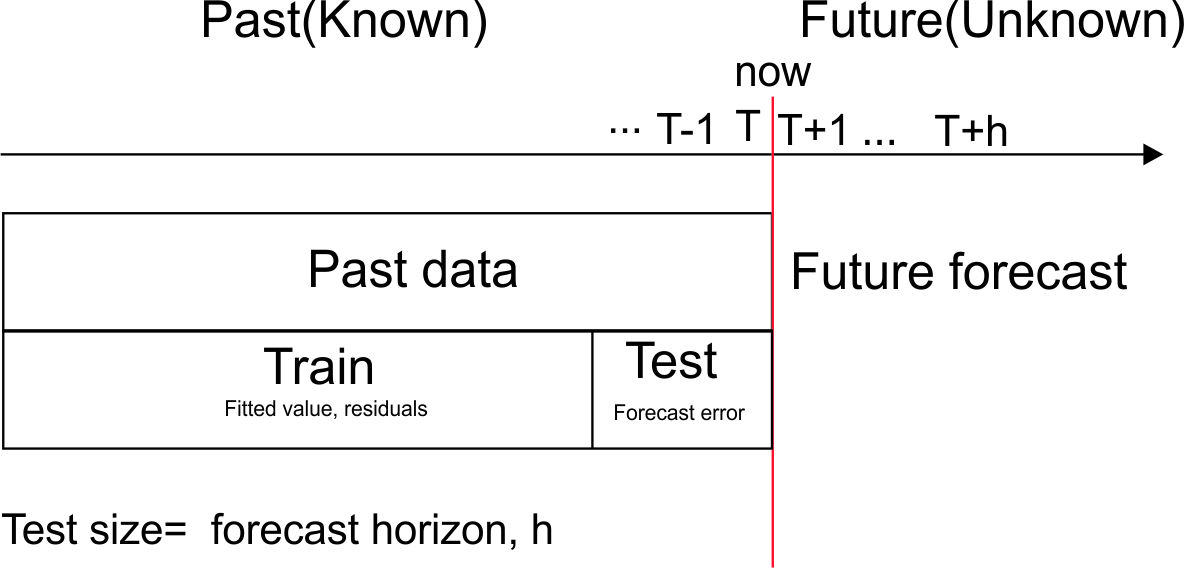
\includegraphics[width=0.9\linewidth,height=\textheight,keepaspectratio]{figs/f_test.jpg}
\end{frame}

\begin{frame}{Time series cross-validation}
\protect\phantomsection\label{time-series-cross-validation-1}
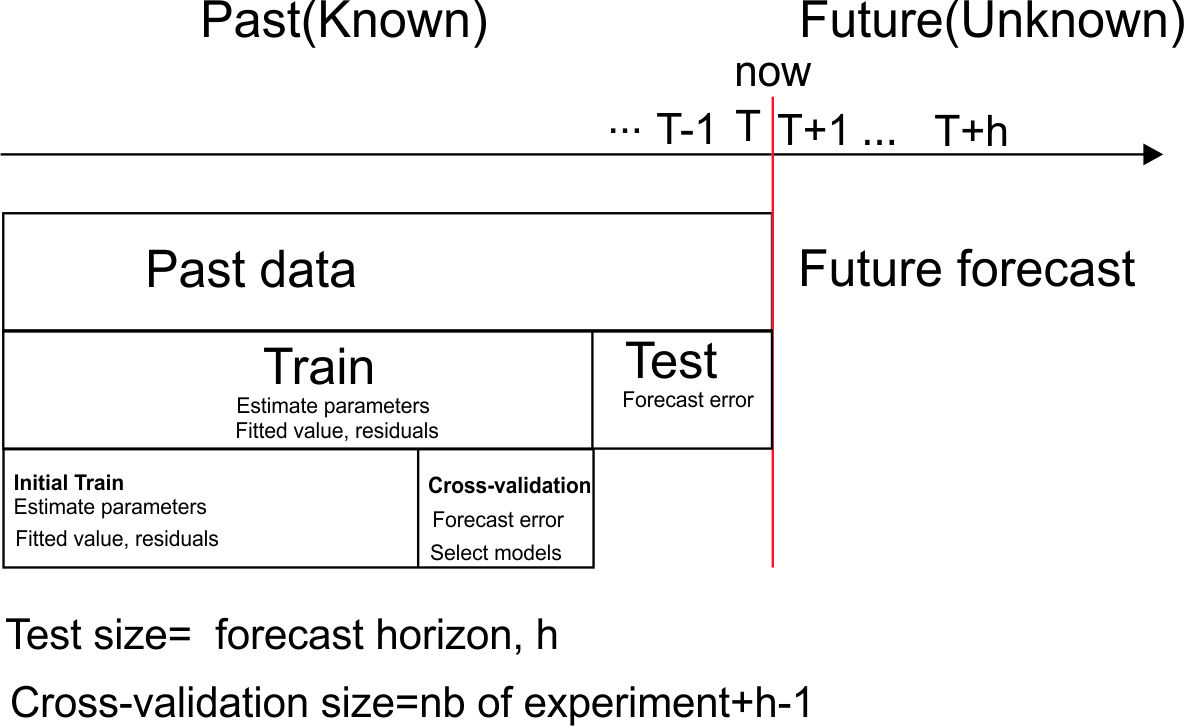
\includegraphics[width=3.95in,height=\textheight,keepaspectratio]{figs/f_future.jpg}
\end{frame}

\begin{frame}{Time series cross-validation}
\protect\phantomsection\label{time-series-cross-validation-2}
\textbf{Time series cross-validation}

\pandocbounded{\includegraphics[keepaspectratio]{05_accuracy_advance_files/figure-beamer/cv1-1.pdf}}

\pause

\begin{itemize}
\tightlist
\item
  Forecast accuracy averaged over test sets.
\item
  Also known as ``evaluation on a rolling forecasting origin''
\end{itemize}

\vspace*{10cm}
\end{frame}

\begin{frame}[fragile]{Creating the rolling training sets}
\protect\phantomsection\label{creating-the-rolling-training-sets}
\fontsize{13}{14}\sf

There are three main rolling types which can be used.

\begin{itemize}
\tightlist
\item
  Stretch: extends a growing length window with new data.
\item
  Slide: shifts a fixed length window through the data.
\item
  Tile: moves a fixed length window without overlap.
\end{itemize}

Three functions to roll a tsibble: \texttt{stretch\_tsibble()},
\texttt{slide\_tsibble()}, and \texttt{tile\_tsibble()}.

For time series cross-validation, stretching windows are most commonly
used.
\end{frame}

\begin{frame}[fragile]{Time series cross-validation}
\protect\phantomsection\label{time-series-cross-validation-3}
\fontsize{12}{13}\sf

Stretch with a minimum length of 24, growing by 1 each step.

\begin{Shaded}
\begin{Highlighting}[]
\NormalTok{forecast\_horizon }\OtherTok{\textless{}{-}} \DecValTok{12}
\NormalTok{test }\OtherTok{\textless{}{-}}\NormalTok{ antidiabetic\_drug\_sale }\SpecialCharTok{|\textgreater{}} 
  \FunctionTok{slice}\NormalTok{((}\FunctionTok{n}\NormalTok{()}\SpecialCharTok{{-}}\NormalTok{forecast\_horizon}\SpecialCharTok{+}\DecValTok{1}\NormalTok{)}\SpecialCharTok{:}\FunctionTok{n}\NormalTok{())}
\NormalTok{train }\OtherTok{\textless{}{-}}\NormalTok{ antidiabetic\_drug\_sale }\SpecialCharTok{|\textgreater{}} 
  \FunctionTok{slice}\NormalTok{(}\DecValTok{1}\SpecialCharTok{:}\NormalTok{(}\FunctionTok{n}\NormalTok{()}\SpecialCharTok{{-}}\NormalTok{forecast\_horizon))}
\NormalTok{drug\_sale\_tcsv }\OtherTok{\textless{}{-}}\NormalTok{  train }\SpecialCharTok{|\textgreater{}} \FunctionTok{slice}\NormalTok{(}\DecValTok{1}\SpecialCharTok{:}\NormalTok{(}\FunctionTok{n}\NormalTok{()}\SpecialCharTok{{-}}\NormalTok{forecast\_horizon)) }\SpecialCharTok{|\textgreater{}} 
  \FunctionTok{stretch\_tsibble}\NormalTok{(}\AttributeTok{.init =} \DecValTok{24}\NormalTok{, }\AttributeTok{.step =} \DecValTok{1}\NormalTok{)}
\end{Highlighting}
\end{Shaded}

\fontsize{10}{11}\sf

\begin{verbatim}
# A tsibble: 2,805 x 3 [1M]
# Key:       .id [55]
     Month  Cost   .id
     <mth> <dbl> <int>
1 2000 Jan 12.5      1
2 2000 Feb  7.46     1
3 2000 Mar  8.59     1
4 2000 Apr  8.47     1
# i 2,801 more rows
\end{verbatim}
\end{frame}

\begin{frame}[fragile]{Time series cross-validation}
\protect\phantomsection\label{time-series-cross-validation-4}
\small

Estimate RW w/ drift models for each window.

\begin{Shaded}
\begin{Highlighting}[]
\NormalTok{drug\_fit\_tr }\OtherTok{\textless{}{-}}\NormalTok{ drug\_sale\_tcsv }\SpecialCharTok{|\textgreater{}} 
  \FunctionTok{model}\NormalTok{(}\AttributeTok{snaive=}\FunctionTok{SNAIVE}\NormalTok{(Cost))}
\end{Highlighting}
\end{Shaded}

\fontsize{10}{11}\sf

\begin{verbatim}
# A mable: 55 x 2
# Key:     .id [55]
    .id   snaive
  <int>  <model>
1     1 <SNAIVE>
2     2 <SNAIVE>
3     3 <SNAIVE>
4     4 <SNAIVE>
# i 51 more rows
\end{verbatim}
\end{frame}

\begin{frame}[fragile]{Time series cross-validation}
\protect\phantomsection\label{time-series-cross-validation-5}
\small

Produce 8 step ahead forecasts from all models.

\begin{Shaded}
\begin{Highlighting}[]
\NormalTok{drug\_fc\_tr }\OtherTok{\textless{}{-}}\NormalTok{ drug\_fit\_tr }\SpecialCharTok{|\textgreater{}} 
  \FunctionTok{forecast}\NormalTok{(}\AttributeTok{h=}\NormalTok{forecast\_horizon)}
\end{Highlighting}
\end{Shaded}

\fontsize{10}{11}\sf

\begin{verbatim}
# A fable: 660 x 5 [1M]
# Key:     .id, .model [55]
    .id .model    Month
  <int> <chr>     <mth>
1     1 snaive 2002 Jan
2     1 snaive 2002 Feb
3     1 snaive 2002 Mar
4     1 snaive 2002 Apr
# i 656 more rows
# i 2 more variables: Cost <dist>, .mean <dbl>
\end{verbatim}
\end{frame}

\begin{frame}[fragile]{Time series cross-validation}
\protect\phantomsection\label{time-series-cross-validation-6}
\small

\begin{Shaded}
\begin{Highlighting}[]
\CommentTok{\# Cross{-}validated}
\NormalTok{drug\_fc\_tr }\SpecialCharTok{|\textgreater{}} 
  \FunctionTok{accuracy}\NormalTok{(antidiabetic\_drug\_sale,}
           \AttributeTok{measures =} \FunctionTok{list}\NormalTok{( point\_accuracy\_measures, }
\NormalTok{                            interval\_accuracy\_measures,}
\NormalTok{                            distribution\_accuracy\_measures))}
\end{Highlighting}
\end{Shaded}

\begin{verbatim}
# A tibble: 1 x 15
  .model .type    ME  RMSE   MAE   MPE  MAPE  MASE RMSSE  ACF1 winkler pinball
  <chr>  <chr> <dbl> <dbl> <dbl> <dbl> <dbl> <dbl> <dbl> <dbl>   <dbl>   <dbl>
1 snaive Test   1.48  1.90  1.56  9.09  9.59  1.17  1.20 0.254    9.73   0.486
# i 3 more variables: scaled_pinball <dbl>, percentile <dbl>, CRPS <dbl>
\end{verbatim}
\end{frame}

\section{Residual diagnostics}\label{residual-diagnostics}

\begin{frame}{Forecasting residuals}
\protect\phantomsection\label{forecasting-residuals}
\begin{block}{}
\textbf{Residuals in forecasting:} difference between observed value and its fitted value: $e_t = y_t-\hat{y}_{t|t-1}$.
\end{block}
\pause\fontsize{13}{15}\sf

\alert{Assumptions}

\begin{enumerate}
\tightlist
\item
  \(\{e_t\}\) uncorrelated. If they aren't, then information left in
  residuals that should be used in computing forecasts.
\item
  \(\{e_t\}\) have mean zero. If they don't, then forecasts are biased.
\end{enumerate}

\pause

\alert{Useful properties} (for prediction intervals)

\begin{enumerate}
\setcounter{enumi}{2}
\tightlist
\item
  \(\{e_t\}\) have constant variance.
\item
  \(\{e_t\}\) are normally distributed.
\end{enumerate}
\end{frame}

\begin{frame}[fragile]{Facebook closing stock price}
\protect\phantomsection\label{facebook-closing-stock-price}
\fontsize{9}{10}\sf

\begin{Shaded}
\begin{Highlighting}[]
\NormalTok{fb\_stock }\OtherTok{\textless{}{-}}\NormalTok{ gafa\_stock }\SpecialCharTok{|\textgreater{}}
  \FunctionTok{filter}\NormalTok{(Symbol }\SpecialCharTok{==} \StringTok{"FB"}\NormalTok{)}
\NormalTok{fb\_stock }\SpecialCharTok{|\textgreater{}} \FunctionTok{autoplot}\NormalTok{(Close)}
\end{Highlighting}
\end{Shaded}

\pandocbounded{\includegraphics[keepaspectratio]{05_accuracy_advance_files/figure-beamer/fbf-1.pdf}}
\end{frame}

\begin{frame}[fragile]{Facebook closing stock price}
\protect\phantomsection\label{facebook-closing-stock-price-1}
\fontsize{10}{10}\sf

\begin{Shaded}
\begin{Highlighting}[]
\NormalTok{fb\_stock }\OtherTok{\textless{}{-}}\NormalTok{ fb\_stock }\SpecialCharTok{|\textgreater{}}
  \FunctionTok{mutate}\NormalTok{(}\AttributeTok{trading\_day =} \FunctionTok{row\_number}\NormalTok{()) }\SpecialCharTok{|\textgreater{}}
  \FunctionTok{update\_tsibble}\NormalTok{(}\AttributeTok{index =}\NormalTok{ trading\_day, }\AttributeTok{regular =} \ConstantTok{TRUE}\NormalTok{)}
\NormalTok{fit }\OtherTok{\textless{}{-}}\NormalTok{ fb\_stock }\SpecialCharTok{|\textgreater{}} \FunctionTok{model}\NormalTok{(}\FunctionTok{NAIVE}\NormalTok{(Close))}
\FunctionTok{augment}\NormalTok{(fit)}
\end{Highlighting}
\end{Shaded}

\begin{verbatim}
# A tsibble: 1,258 x 7 [1]
# Key:       Symbol, .model [1]
   Symbol .model       trading_day Close .fitted .resid .innov
   <chr>  <chr>              <int> <dbl>   <dbl>  <dbl>  <dbl>
 1 FB     NAIVE(Close)           1  54.7    NA   NA     NA    
 2 FB     NAIVE(Close)           2  54.6    54.7 -0.150 -0.150
 3 FB     NAIVE(Close)           3  57.2    54.6  2.64   2.64 
 4 FB     NAIVE(Close)           4  57.9    57.2  0.720  0.720
 5 FB     NAIVE(Close)           5  58.2    57.9  0.310  0.310
 6 FB     NAIVE(Close)           6  57.2    58.2 -1.01  -1.01 
 7 FB     NAIVE(Close)           7  57.9    57.2  0.720  0.720
 8 FB     NAIVE(Close)           8  55.9    57.9 -2.03  -2.03 
 9 FB     NAIVE(Close)           9  57.7    55.9  1.83   1.83 
10 FB     NAIVE(Close)          10  57.6    57.7 -0.140 -0.140
# i 1,248 more rows
\end{verbatim}
\end{frame}

\begin{frame}[fragile]{Facebook closing stock price}
\protect\phantomsection\label{facebook-closing-stock-price-2}
\fontsize{10}{10}\sf

\begin{Shaded}
\begin{Highlighting}[]
\FunctionTok{augment}\NormalTok{(fit) }\SpecialCharTok{|\textgreater{}}
  \FunctionTok{ggplot}\NormalTok{(}\FunctionTok{aes}\NormalTok{(}\AttributeTok{x =}\NormalTok{ trading\_day)) }\SpecialCharTok{+}
  \FunctionTok{geom\_line}\NormalTok{(}\FunctionTok{aes}\NormalTok{(}\AttributeTok{y =}\NormalTok{ Close, }\AttributeTok{colour =} \StringTok{"Data"}\NormalTok{)) }\SpecialCharTok{+}
  \FunctionTok{geom\_line}\NormalTok{(}\FunctionTok{aes}\NormalTok{(}\AttributeTok{y =}\NormalTok{ .fitted, }\AttributeTok{colour =} \StringTok{"Fitted"}\NormalTok{))}
\end{Highlighting}
\end{Shaded}

\pandocbounded{\includegraphics[keepaspectratio]{05_accuracy_advance_files/figure-beamer/dj4-1.pdf}}
\end{frame}

\begin{frame}[fragile]{Facebook closing stock price}
\protect\phantomsection\label{facebook-closing-stock-price-3}
\fontsize{10}{10}\sf

\begin{Shaded}
\begin{Highlighting}[]
\FunctionTok{augment}\NormalTok{(fit) }\SpecialCharTok{|\textgreater{}}
  \FunctionTok{filter}\NormalTok{(trading\_day }\SpecialCharTok{\textgreater{}} \DecValTok{1100}\NormalTok{) }\SpecialCharTok{|\textgreater{}}
  \FunctionTok{ggplot}\NormalTok{(}\FunctionTok{aes}\NormalTok{(}\AttributeTok{x =}\NormalTok{ trading\_day)) }\SpecialCharTok{+}
  \FunctionTok{geom\_line}\NormalTok{(}\FunctionTok{aes}\NormalTok{(}\AttributeTok{y =}\NormalTok{ Close, }\AttributeTok{colour =} \StringTok{"Data"}\NormalTok{)) }\SpecialCharTok{+}
  \FunctionTok{geom\_line}\NormalTok{(}\FunctionTok{aes}\NormalTok{(}\AttributeTok{y =}\NormalTok{ .fitted, }\AttributeTok{colour =} \StringTok{"Fitted"}\NormalTok{))}
\end{Highlighting}
\end{Shaded}

\pandocbounded{\includegraphics[keepaspectratio]{05_accuracy_advance_files/figure-beamer/dj4a-1.pdf}}
\end{frame}

\begin{frame}[fragile]{Facebook closing stock price}
\protect\phantomsection\label{facebook-closing-stock-price-4}
\fontsize{10}{10}\sf

\begin{Shaded}
\begin{Highlighting}[]
\FunctionTok{augment}\NormalTok{(fit) }\SpecialCharTok{|\textgreater{}}
  \FunctionTok{autoplot}\NormalTok{(.resid) }\SpecialCharTok{+}
  \FunctionTok{labs}\NormalTok{(}\AttributeTok{x =} \StringTok{"Day"}\NormalTok{, }\AttributeTok{y =} \StringTok{""}\NormalTok{, }\AttributeTok{title =} \StringTok{"Residuals from naïve method"}\NormalTok{)}
\end{Highlighting}
\end{Shaded}

\pandocbounded{\includegraphics[keepaspectratio]{05_accuracy_advance_files/figure-beamer/dj5-1.pdf}}
\end{frame}

\begin{frame}[fragile]{Facebook closing stock price}
\protect\phantomsection\label{facebook-closing-stock-price-5}
\fontsize{11}{11}\sf

\begin{Shaded}
\begin{Highlighting}[]
\FunctionTok{augment}\NormalTok{(fit) }\SpecialCharTok{|\textgreater{}}
  \FunctionTok{ggplot}\NormalTok{(}\FunctionTok{aes}\NormalTok{(}\AttributeTok{x =}\NormalTok{ .resid)) }\SpecialCharTok{+}
  \FunctionTok{geom\_histogram}\NormalTok{(}\AttributeTok{bins =} \DecValTok{150}\NormalTok{) }\SpecialCharTok{+}
  \FunctionTok{labs}\NormalTok{(}\AttributeTok{title =} \StringTok{"Histogram of residuals"}\NormalTok{)}
\end{Highlighting}
\end{Shaded}

\pandocbounded{\includegraphics[keepaspectratio]{05_accuracy_advance_files/figure-beamer/dj6-1.pdf}}
\end{frame}

\begin{frame}[fragile]{Facebook closing stock price}
\protect\phantomsection\label{facebook-closing-stock-price-6}
\fontsize{11}{11}\sf

\begin{Shaded}
\begin{Highlighting}[]
\FunctionTok{augment}\NormalTok{(fit) }\SpecialCharTok{|\textgreater{}}
  \FunctionTok{ACF}\NormalTok{(.resid) }\SpecialCharTok{|\textgreater{}}
  \FunctionTok{autoplot}\NormalTok{() }\SpecialCharTok{+} \FunctionTok{labs}\NormalTok{(}\AttributeTok{title =} \StringTok{"ACF of residuals"}\NormalTok{)}
\end{Highlighting}
\end{Shaded}

\pandocbounded{\includegraphics[keepaspectratio]{05_accuracy_advance_files/figure-beamer/dj7-1.pdf}}
\end{frame}

\begin{frame}{ACF of residuals}
\protect\phantomsection\label{acf-of-residuals}
\begin{itemize}
\item
  We assume that the residuals are white noise (uncorrelated, mean zero,
  constant variance). If they aren't, then there is information left in
  the residuals that should be used in computing forecasts.
\item
  So a standard residual diagnostic is to check the ACF of the residuals
  of a forecasting method.
\item
  We \emph{expect} these to look like white noise.
\end{itemize}
\end{frame}

\begin{frame}[fragile]{Combined diagnostic graph}
\protect\phantomsection\label{combined-diagnostic-graph}
\fontsize{11}{11}\sf

\begin{Shaded}
\begin{Highlighting}[]
\NormalTok{fit }\SpecialCharTok{|\textgreater{}} \FunctionTok{gg\_tsresiduals}\NormalTok{()}
\end{Highlighting}
\end{Shaded}

\pandocbounded{\includegraphics[keepaspectratio]{05_accuracy_advance_files/figure-beamer/dj8-1.pdf}}
\end{frame}

\begin{frame}{Ljung-Box test}
\protect\phantomsection\label{ljung-box-test}
\fontsize{12}{13}\sf

Test whether \emph{whole set} of \(r_{k}\) values is significantly
different from zero set.

\begin{block}{}
\centerline{$\displaystyle
 Q = T(T+2) \sum_{k=1}^\ell (T-k)^{-1}r_k^2$\qquad
where $\ell=$ max lag and $T=$ \# observations}
\end{block}

\begin{itemize}
\tightlist
\item
  If each \(r_k\) close to zero, \(Q\) will be \textbf{small}.
\item
  If some \(r_k\) values large (\(+\) or \(-\)), \(Q\) will be
  \textbf{large}.
\item
  My preferences: \(h=10\) for non-seasonal data, \(h=2m\) for seasonal
  data.
\item
  If data are WN and \(T\) large, \(Q \sim \chi^2\) with \(\ell\)
  degrees of freedom.
\end{itemize}
\end{frame}

\begin{frame}[fragile]{Ljung-Box test}
\protect\phantomsection\label{ljung-box-test-1}
\fontsize{12}{13}\sf

\begin{block}{}
\centerline{$\displaystyle
 Q = T(T+2) \sum_{k=1}^\ell (T-k)^{-1}r_k^2$\qquad
where $\ell=$ max lag and $T=$ \# observations.}
\end{block}

\fontsize{11}{11}\sf

\pandocbounded{\includegraphics[keepaspectratio]{05_accuracy_advance_files/figure-beamer/dj9extra-1.pdf}}

\vspace*{-0.3cm}

\begin{Shaded}
\begin{Highlighting}[]
\CommentTok{\# lag = h}
\FunctionTok{augment}\NormalTok{(fit) }\SpecialCharTok{|\textgreater{}} \FunctionTok{features}\NormalTok{(.resid, ljung\_box, }\AttributeTok{lag =} \DecValTok{10}\NormalTok{)}
\end{Highlighting}
\end{Shaded}

\begin{verbatim}
# A tibble: 1 x 4
  Symbol .model       lb_stat lb_pvalue
  <chr>  <chr>          <dbl>     <dbl>
1 FB     NAIVE(Close)    12.1     0.276
\end{verbatim}
\end{frame}

\section{Recap}\label{recap}

\begin{frame}[fragile]{Recap}
\protect\phantomsection\label{recap-1}
\fontsize{12}{12}\sf

\begin{enumerate}
\tightlist
\item
  First, import your data and prepare them using \texttt{tsibble}
  function.
\item
  Visualise and see whether your series contains key patetrns Use domain
  knowledge to understand your data and potential driving factors.
\item
  Split the data to create a training set, which you will use as an
  argument in your forecasting function(s). You can also create a test
  set to use later.
\item
  Create different rolling origins to evaluate forecast accuracy using
  time series cross validation
\end{enumerate}
\end{frame}

\begin{frame}[fragile]{Recap}
\protect\phantomsection\label{recap-2}
\fontsize{12}{12}\sf

\begin{enumerate}
\setcounter{enumi}{4}
\tightlist
\item
  Train model to each origin
\item
  Computer forecast accuracy, use the \texttt{accuracy()} function with
  the \texttt{fable} as the first argument and original data as the
  second.
\item
  Compare methods using point, prediction interval and distributional
  accuracy measure; a smaller error indicates higher accuracy.
\item
  Forecast using all data for the future using the best method.
\item
  Use residual diagnostic based on residuals of the best model.
\end{enumerate}
\end{frame}




\end{document}
